\documentclass{beamer}
\beamertemplatenavigationsymbolsempty
\usecolortheme{beaver}
\setbeamertemplate{blocks}[rounded=true, shadow=true]
\setbeamertemplate{footline}[page number]
%
\usepackage[utf8]{inputenc}
\usepackage[english,russian]{babel}
\usepackage{amssymb,amsfonts,amsmath,mathtext}
\usepackage{subfig}
\usepackage[all]{xy} % xy package for diagrams
\usepackage{array}
\usepackage{multicol}% many columns in slide
\usepackage{hyperref}% urls
\usepackage{hhline}%tables
\usepackage{ dsfont }

% Your figures are here:
\graphicspath{ {fig/} {../fig/} }

%----------------------------------------------------------------------------------------------------------
\title[\hbox to 56mm{Порождение признаков}]{Выбор согласованных моделей для \\ построения нейроинтерфейса}
\author[Я. Кулаков]{Кулаков Ярослав Михайлович}
\institute{Московский физико-технический институт}
\date{\footnotesize
\par\smallskip\emph{Курс:} Автоматизация научных исследований\par (практика, В.\,В.~Стрижов)/Группа 813
\par\smallskip\emph{Эксперт:} В~.Стрижов
\par\smallskip\emph{Консультант:} Р.~Исаченко
\par\bigskip\small 2021}
%----------------------------------------------------------------------------------------------------------
\begin{document}
%----------------------------------------------------------------------------------------------------------
\begin{frame}
\thispagestyle{empty}
\maketitle
\end{frame}
%-----------------------------------------------------------------------------------------------------

%-----------------------------------------------------------------------------------------------------

\begin{frame}{Прогнозирование координаты кисти по сигналам электрокортикограммы ECoG}

$(X, Y).$ $ X \in \mathds{R}^{T, K}$, где $T$ --- количество временных отметок,\\
$K$ ---  количество электродов,\\
$Y \in \mathds{R}^{C, T}$, где $C$ --- номер координаты в трехмерном пространстве.

\begin{columns}[c]
\column{0.9\textwidth}
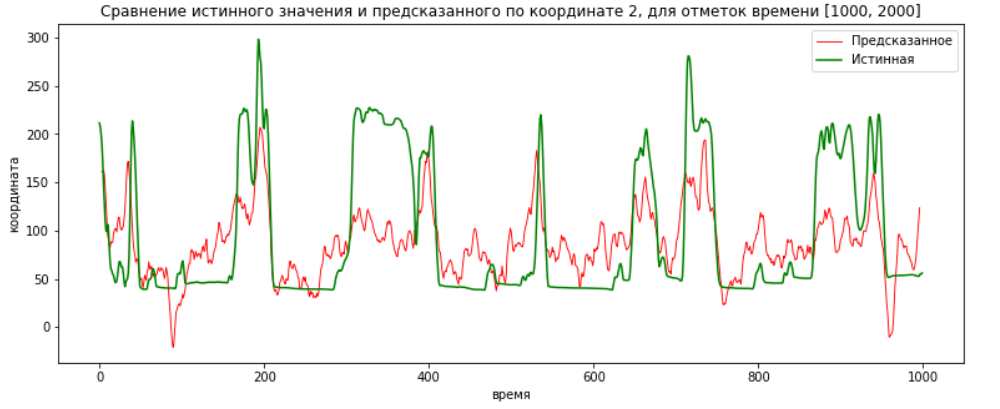
\includegraphics[width=1.0\textwidth]{images/predicted_actual_coords}

%    Столбец 1
%\column{0.4\textwidth}
%    Столбец 2
\end{columns}

\bigskip

Линейный {\color{red}PLS} хорошо предсказывает пики, но плохо константные области.
\end{frame}


%----------------------------------------------------------------------------------------------------------
\end{document} 